%!TEX root = Main.tex
\section*{Gaussian Mixture Models}
Gaussian Mixture Models (GMM) is a way of finding and describing sub-populations in clusters of data points.
It is done by fitting a specified number of Gaussian distributions to a population of data points.
Each distribution is a component of the model. 
The individual data points are then arranged into clusters based on which model component is most likely given the observed data point.

The distributions of the mixture model are fitted to data by iteratively employing Expectation Maximization (EM).

\subsection*{The EM Algotrithm}
In EM a mixture model is iteratively updated by estimating model parameters $\bm{\mu}_k $ \emph{component means} (\ref{eq:GMM_mu}) and $ \bm{\Sigma}_k $ \emph{component covariance matrix} (\ref{eq:GMM_Sigma}) based on current assignment of responsibility and then reassigning responsibility based on new model parameters (\ref{eq:GMM_gamma}), starting out with a random guess of $\bm{\mu}_k \text{ and } \bm{\Sigma}_k \text{ for } k=1..K$ 


\subsubsection*{Initialization:}
\begin{enumerate}
\item
Choose initial estimates for model parameters $ \mathbf{\pi}_{k}, \mathbf{\mu}_{k}, \mathbf{\Sigma}_{k} $.

\begin{itemize}

	\item
	$ k $ is the component number out of K.

	\item
	$ \pi_{k} $  is the weight of the \textit{k}th component.

	\item
	$ \mathbf{\mu}_{k}$ is the mean of the \textit{k}th component.

	\item
	$ \mathbf{\Sigma}_{k} $ is the covariance matrix of the \textit{k}th component.

	\end{itemize}


\item
Compute the initial log-likelihood og the model

\begin{equation} \label{eq:loglikeGMM}
\ln p\left(X | \mathbf{\mu}, \mathbf{\Sigma}, \pi\right) = 
\sum_{n=1}^{N} \ln \sum_{k=1}^{N} \pi_{k}\mathcal{N}(\mathbf{x}_{n}|\mathbf{\mu}_{k},\mathbf{\Sigma}_{k})
\end{equation}

\end{enumerate}

\subsubsection*{E-step:}
Calculate the probability of each point in each component in order to assign responsibility

\begin{equation}
\label{eq:GMM_gamma} 
\gamma_{nk} = 
\frac
{\pi_{k}\mathcal{N}(\mathbf{x}_{n}|\mathbf{\mu}_{k},\mathbf{\Sigma}_{k})}
{\sum_{j=1}^{K} \pi_{n}\mathcal{N}(\mathbf{x}_{n}|\mu_{j},\mathbf{\Sigma}_{j})}
\end{equation}

\subsubsection*{M-step:}
Estimate new guesses for $ \mathbf{\pi}_{k}, \bm{\mu}_{k}, \bm{\Sigma}_{k} $.

\begin{equation}
\label{eq:GMM_mu} 
\bm{\mu}_{k}^{new} = 
\frac{1}{N_{k}}
\sum_{n=1}^{N} 
\gamma_{nk}
\mathbf{x}_{k}
\end{equation}

\begin{equation}
\label{eq:GMM_Sigma} 
\bm{\Sigma}_{k}^{new} = 
\frac{1}{N_{k}}
\sum_{n=1}^{N} 
\gamma_{nk}
(\mathbf{x}_{k} - \bm{\mu}_{k}^{new})
(\mathbf{x}_{k} - \bm{\mu}_{k}^{new})^{T}
\end{equation}

\begin{equation}
\pi_{k}^{new} =
\frac
{N_{k}}
{N}
\end{equation}

\subsubsection*{Convergence check:}

Recalculate log likelihood using (\ref{eq:loglikeGMM}).
If the log likelihood has not changed more than some predetermined threshold stop iteration.
Otherwise continue from E-step.

\subsection*{Training}
GMM is a type of unsupervised machine learning, and is a first hand not useful in our project, but by training a GMM for each speaker based on the pre-classified training set, you end up with a very effective model.
When applied in this way the components of the individual speaker models can be thought of as a PGM for each characteristic sound a speaker makes.
Combined into a mixture model, these components make up a accurate and narrow model of an individual speakers voice.
This allows for speaker classification on the basis of highest overall likelihood.

To further improve classification, overall likelihood is averaged, for each speaker model, over a superframe of 100 frames.
This is done on the assumption that only one speaker is speaking at a time, so this speakers model is most likely to have the greatest overall likelihood for most frames out of the superframe.

\subsection*{Results}
\begin{figure}[H]
\centering
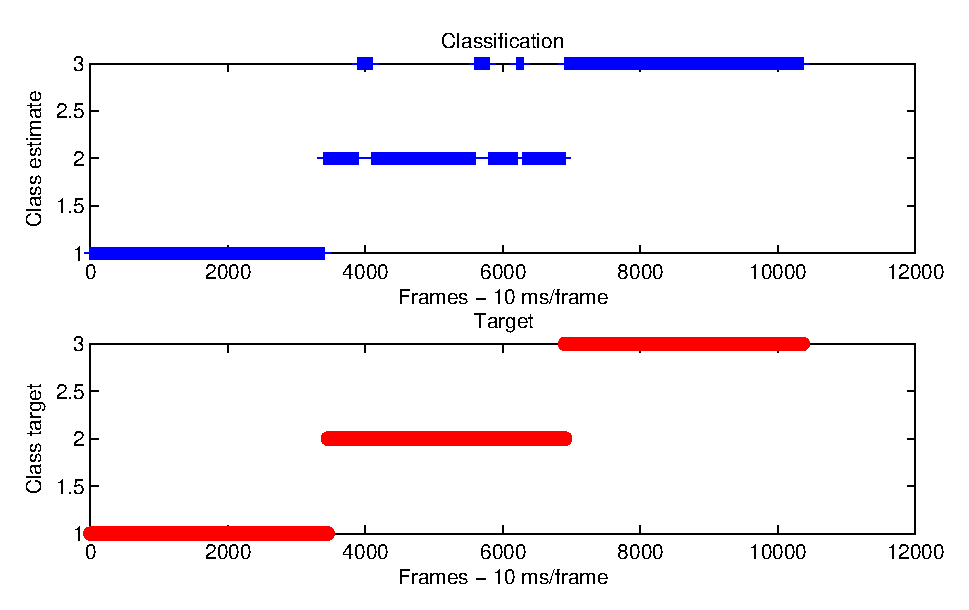
\includegraphics[width=\linewidth]{GMM_1digit_8cent_3speak}
\caption{Results of using GMM with 3 speakers, 8 centers per model and 1 digit spoken}
\label{fig:GMM_fig_1}
\end{figure}

Gaussian Mixture Models with a trained model for each speaker yielded a very high classification accuracy. $  94.6\ \%, 91.2\ \% \text{ and }  89.1\ \% $ for 1, 2 and 10 digits spoken, respectively.
The estimated for one digit is shown on figure \ref{fig:GMM_fig_1}, where the the blue is the estimated. 


